% arara: lualatex: { interaction: nonstopmode, synctex: no }
% arara: lualatex: { interaction: nonstopmode, synctex: no }
\documentclass[a4paper,12pt,chapterprefix=false,bibliography=totoc,listof=totoc,book]{scrreprt}

\usepackage{latex-style}

\lstdefinelanguage{Gherkin}{
	morekeywords = {
		Given,
		When,
		Then,
		And,
		Scenario,
		Feature,
		But,
		Background,
		Scenario Outline,
		Examples
	},
	sensitive=true,
	morecomment=[l]{\#},
	morestring=[b]",
	morestring=[b]',
	keywordstyle=\normalsize\bfseries\color{green},
	basicstyle=\small\ttfamily,
}

\setlength{\parindent}{0pt}

\begin{document}
\begin{flushright}
GameBase
\\
Use-Case Specification: Create GameServer
% \\
% For <Subsystem or Feature>
\bigbreak
Version 1.0
\end{flushright}

\tableofcontents

\chapter{Use-Case: Create GameServer}

\section{Brief Description}
The use case describes the creation of gameservers

\chapter{Flow of Events}
\begin{figure}[H]
	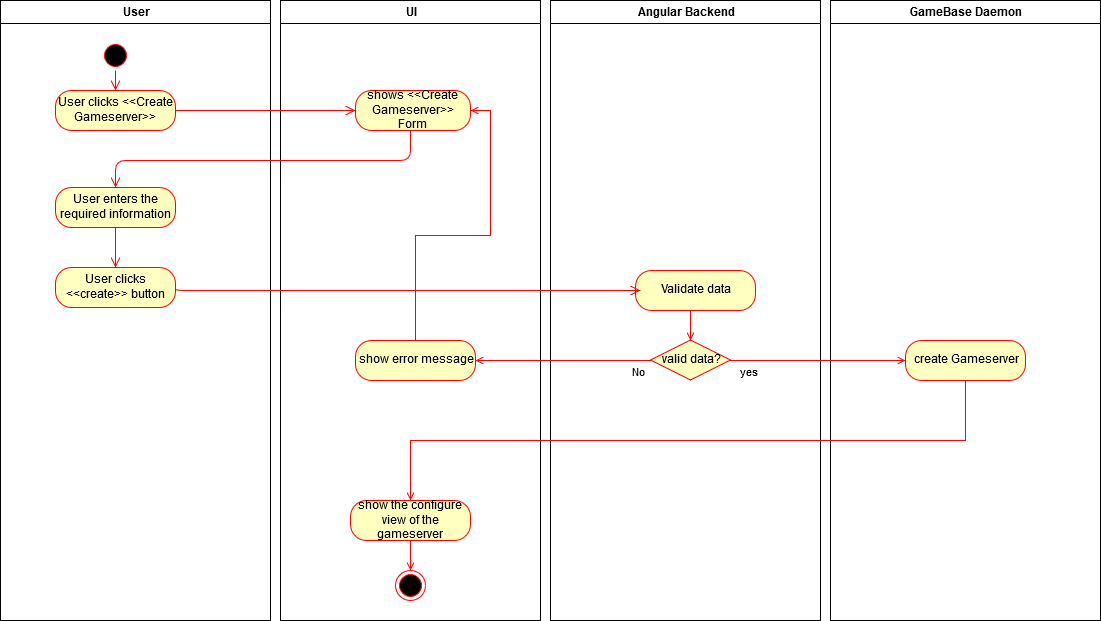
\includegraphics[width=\textwidth]{diagramms/CreateGameserverActivityDiagramm.png}
	\caption{Activity Diagramm}
	\label{fig:ucd}
\end{figure}
\section{Basic flow}

\begin{itemize}
    \item User clicks on <<Create GameServer>>
    \item User fills the form with the required information
    \item User clicks on <<Create>> to create the GameServer and gets redirected to the gameservers configuration page
    \item or the User clicks on <<Cancel>> to cancel the Create operation
\end{itemize}


\section{.feature File}
\lstinputlisting[language=Gherkin]{features/createGameServer.feature}


\section{Creation}
[include image]\\
The creation of a new gameserver. The user will be asked to select the type (game) of the gamserver.

\chapter{Special Requirements}

\section{Owning an account}
The user has to be a registered user for our system.

\chapter{Preconditions}
\section{Must be logged in}
The user must be logged in to create, edit, see or delete a server.

\chapter{Postconditions}

\section{Create}
After creating the gameserver the user will be redirected to the gameservers configuration page to set all required configuration options for that server.

\end{document}